\documentclass[12pt]{article}

% \usepackage{extsizes}  % 字體文件使用 14pt
\usepackage{CJKutf8}
\usepackage[margin=2.0cm]{geometry}
\usepackage{fancyhdr}  % 頁首、頁尾
\usepackage{graphicx}
\usepackage{amsmath, amssymb, amsfonts}
\usepackage{listings}  % code showing
\usepackage{pagecolor}  % for code color define
\usepackage{tocloft}  % contents

% -- 格式
\pagestyle{fancy}  % 使用 header
\fancyhf{}
\setcounter{secnumdepth}{-1}  % 移除 section 數字
\renewcommand{\cftsecleader}{\cftdotfill{\cftdotsep}}

%% -- 標題使用中文取代
\renewcommand{\figurename}{圖}
\renewcommand{\tablename}{表}
\renewcommand{\lstlistingname}{程式碼}

%% -- 間距設定
% \linespread{1.2}\selectfont  % 行距
\setlength{\headheight}{29pt}
\setlength\parindent{0pt}
\setlength{\parskip}{0.5em}
\setlength{\abovecaptionskip}{10pt}  % 圖表標題 caption 與圖表的距離
\setlength{\belowcaptionskip}{10pt}

% -- 顯示程式碼格式
\definecolor{codegreen}{rgb}{0,0.6,0}
\definecolor{codegray}{rgb}{0.5,0.5,0.5}
\definecolor{codepurple}{rgb}{0.58,0,0.82}
\definecolor{backcolour}{rgb}{0.95,0.95,0.92}
\lstdefinestyle{pystyle}{
    backgroundcolor=\color{backcolour},
    commentstyle=\color{codegreen},
    keywordstyle=\color{magenta},
    numberstyle=\footnotesize\color{codegray},
    stringstyle=\color{codepurple},
    basicstyle=\ttfamily\footnotesize,
    breakatwhitespace=false,
    breaklines=true,
    captionpos=b,
    keepspaces=true,
    numbers=left,
    numbersep=5pt,
    showspaces=false,
    showstringspaces=false,
    showtabs=false,
    tabsize=2,
    extendedchars=false
}



\lstset{style=pystyle}
% ---------------------------------------------

\begin{document}
\begin{CJK}{UTF8}{bkai}

\chead{\normalsize \textbf{Homework }}  % 可調整大小
\lhead{\normalsize 10-Bar Truss Optimization}
\rhead{\normalsize R11522637 柯琮祐}
\cfoot{\thepage}

\tableofcontents\thispagestyle{fancy}

% ---------------------------------------------

\section{Problem }

問題描述\\

\begin{figure}[h]
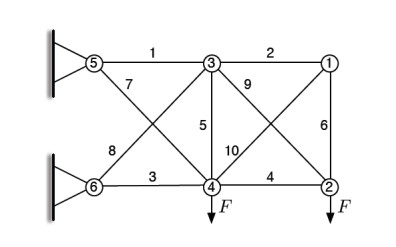
\includegraphics[scale=1.0]{./graph/10bar.jpg}
\end{figure}

在以下的已知條件下,給定桿件截面半徑,利用有限元素分析法求各桿件的位移、應力與反作用力:\\
 • 整體架構處在靜力平衡的情況下\\
 • 所有桿件截面皆為圓形\\
 • 材料為鋼,楊氏係數 E = 200 GPa,密度 ρ = 7860 kg/m3,降伏強度 σy = 250 MPa\\
 • 平行桿件與鉛直桿件(桿件1至桿件6)長度皆為 9.14 m\\
 • 桿件 1 至桿件 6 截面半徑相同為 r1,桿件 7 至桿件 10 截面半徑相同為 r2\\
 • 所有桿件半徑的最佳化範圍為 0.001 至 0.5 m 之間\\
 • 在節點 2 和節點 4 上的負載 F 皆為 1.0 × 107 N 向下\\
 
並在以下條件下最佳化桿件的總重量及桿件半徑\\

\begin{align}
    min_{r1,r2} \quad  f(r1,r2)&= \sum_{i=1}^{6} m_i(r1)+ \sum_{i=7}^{10} m_i(r2)\\
    subject \ to \left| \sigma i \right| &\leq \sigma y\\
    \Delta _{s2} &\leq 0.02\\
     where f&:\mbox{所有桿件質量}\\
 	\Delta _{s2}&:node 2\mbox{位移}\\
 	\sigma y&:\mbox{降伏應力}\\
	\sigma i&:\mbox{所有桿件應力}\
\end{align}
 。




\subsection*{Solution}

\textbf{Step1.有限元素分析法程式建立:用以計算所有桿件應力、應變及反作用力}:參考了orientation上建立了3個fuction來處理有限元素法。\\


跟著orientation上的提示先定義各參數數值,參考pdf中element table 2-2,先建立node矩陣記錄了個節點的x及y座標。
並輸入楊氏係數E。
\begin{lstlisting}
	function [sigma, Q] = sol_TenBarTruss(r1, r2)
	%定義各參數數值
	E=200*10^9;。
    node=[18.28,9.14;18.28,0;9.14,9.14;9.14,0;0,9.14;0,0];
\end{lstlisting}
參考pdf中element table 2-3輸入計算剛性矩陣所需的桿件面積A,桿件長度L及桿件夾角theta(角度部分原本使用pdf中的公式後acos但角度常常不對導致剛性矩陣錯誤所以最後使用acot計算。
\begin{lstlisting}
    A=zeros(10,1);
    A(1:6,1)=r1^2*pi();
    A(7:10,1)=r2^2*pi();
    L=zeros(10,1);
    L(1,1)=sqrt((node(5,1)-node(3,1))^2+(node(5,2)-node(3,2))^2);
    L(2,1)=sqrt((node(3,1)-node(1,1))^2+(node(3,2)-node(1,2))^2);
    L(3,1)=sqrt((node(6,1)-node(4,1))^2+(node(6,2)-node(4,2))^2); 
    L(4,1)=sqrt((node(4,1)-node(2,1))^2+(node(4,2)-node(2,2))^2);
    L(5,1)=sqrt((node(4,1)-node(3,1))^2+(node(4,2)-node(3,2))^2);
    L(6,1)=sqrt((node(2,1)-node(1,1))^2+(node(2,2)-node(1,2))^2);
    L(7,1)=sqrt((node(5,1)-node(4,1))^2+(node(5,2)-node(4,2))^2);
    L(8,1)=sqrt((node(6,1)-node(3,1))^2+(node(6,2)-node(3,2))^2);
    L(9,1)=sqrt((node(3,1)-node(2,1))^2+(node(3,2)-node(2,2))^2);
    L(10,1)=sqrt((node(4,1)-node(1,1))^2+(node(4,2)-node(1,2))^2);
    theta=zeros(10,1);
    theta(1,1)=acotd((node(5,1)-node(3,1))/(node(5,2)-node(3,2)));
    theta(2,1)=acotd((node(3,1)-node(1,1))/(node(3,2)-node(1,2)));
    theta(3,1)=acotd((node(6,1)-node(4,1))/(node(6,2)-node(4,2)));
    theta(4,1)=acotd((node(4,1)-node(2,1))/(node(4,2)-node(2,2)));
    theta(5,1)=acotd((node(4,1)-node(3,1))/(node(4,2)-node(3,2)));
    theta(6,1)=acotd((node(2,1)-node(1,1))/(node(2,2)-node(1,2)));
    theta(7,1)=acotd((node(5,1)-node(4,1))/(node(5,2)-node(4,2)));
    theta(8,1)=acotd((node(6,1)-node(3,1))/(node(6,2)-node(3,2)));
    theta(9,1)=acotd((node(3,1)-node(2,1))/(node(3,2)-node(2,2)));
    theta(10,1)=acotd((node(4,1)-node(1,1))/(node(4,2)-node(1,2)));
\end{lstlisting}
跟著orientation提示先建立K空白矩陣及計算10桿結構之剛性矩陣。
\begin{lstlisting}   
    % 開一個空白的剛性矩陣 (stiffness matrix)
    K=zeros(12);
    % 計算 stiffness matrix (可使用 add_element 函數)
    K = add_element(K,A(1,1),E,L(1,1),theta(1,1),3,5);
    K = add_element(K,A(2,1),E,L(2,1),theta(2,1),1,3);
    K = add_element(K,A(3,1),E,L(3,1),theta(3,1),4,6);
    K = add_element(K,A(4,1),E,L(4,1),theta(4,1),2,4);
    K = add_element(K,A(5,1),E,L(5,1),theta(5,1),3,4);
    K = add_element(K,A(6,1),E,L(6,1),theta(6,1),1,2);
    K = add_element(K,A(7,1),E,L(7,1),theta(7,1),4,5);
    K = add_element(K,A(8,1),E,L(8,1),theta(8,1),3,6);
    K = add_element(K,A(9,1),E,L(9,1),theta(9,1),2,3);
    K = add_element(K,A(10,1),E,L(10,1),theta(10,1),1,4);
\end{lstlisting}
add element 函數與orientation相同為
\begin{lstlisting}
function K = add_element(K, A, E, L, theta, node1, node2)
    c = cosd(theta); s = sind(theta);
    temp = A*E/L*[c^2 c*s; c*s s^2];
    K((2*node1-1):(2*node1), (2*node1-1):(2*node1))...
    = K((2*node1-1):(2*node1), (2*node1-1):(2*node1)) + temp;
    K((2*node2-1):(2*node2), (2*node2-1):(2*node2))...
    = K((2*node2-1):(2*node2), (2*node2-1):(2*node2)) + temp;
    K((2*node1-1):(2*node1), (2*node2-1):(2*node2))...
    = K((2*node1-1):(2*node1), (2*node2-1):(2*node2)) - temp;
    K((2*node2-1):(2*node2), (2*node1-1):(2*node1))...
    = K((2*node2-1):(2*node2), (2*node1-1):(2*node1)) - temp;
end
\end{lstlisting}

透過檔案TESTK.m跑r1=0.1(m),r2=0.05(m)的情況確保剛性矩陣正確\\
\begin{figure}[h]
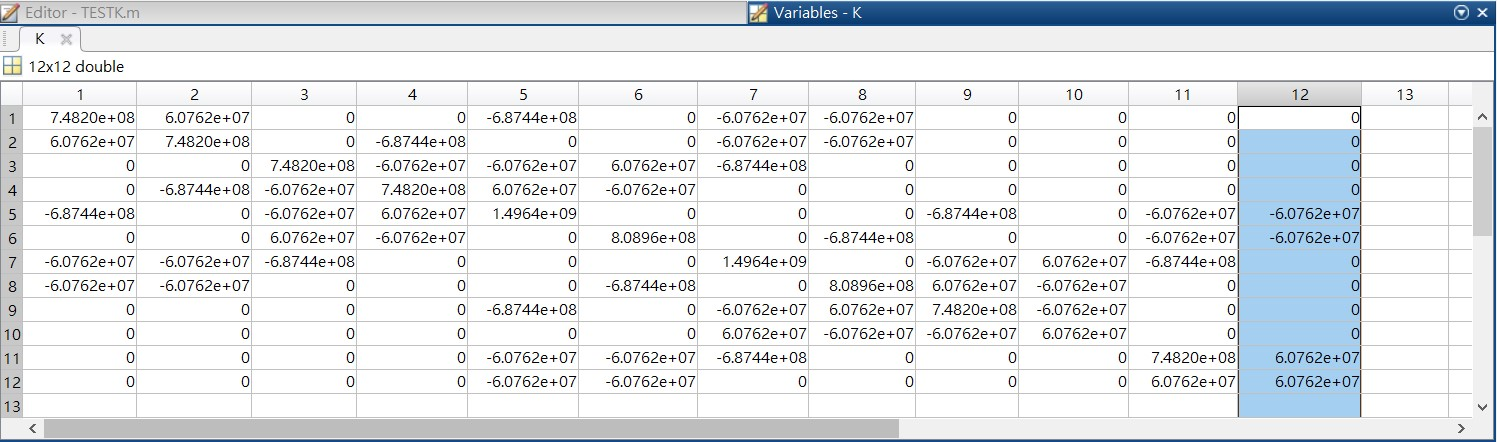
\includegraphics[scale=0.5]{./graph/KTEST.jpg}
\end{figure}

接著建立力矩陣,題目施加了2個力分別在節點2和節點4的-y方向因此力矩陣的為下,Fr為Freduced根據manual節點5.6為固定端計算位移矩陣用不到所以計算位移矩陣只需用到Fr。
\begin{lstlisting}
% 建立力矩陣
	F=[0 0 0 -1*10^7 0 0 0 -1*10^7 0 0 0 0]';
    Fr=F(1:8,1);
\end{lstlisting}

最後建立空白位移及應力矩陣後,計算應力、應變及反作用力完成有限元素分析法部分,Qr為Qreduced原因跟Fr一樣,QF為用來計算反作用力時使用沒有將節點5.6位移歸零,compute stress程式與orietation相同。

\begin{lstlisting}
	% 建立空白位移矩陣
    Q =zeros(12,1);
  
    % 計算位移量 (F = KQ)
    Kr=K(1:8,1:8);
    %QF=inv(K)*F;
    Qr= inv(Kr)*Fr;
    Q(1:8,1)=Qr;
    % 建立空白應力矩陣
    sigma = zeros(10,1);
  
    % 計算應力 (stress) (可使用 compute_stress 函數)
    sigma(1,1)= compute_stress(Q,E,L(1,1),theta(1,1),3,5);
    sigma(2,1)= compute_stress(Q,E,L(2,1),theta(2,1),1,3);
    sigma(3,1)= compute_stress(Q,E,L(3,1),theta(3,1),4,6);
    sigma(4,1)= compute_stress(Q,E,L(4,1),theta(4,1),2,4);
    sigma(5,1)= compute_stress(Q,E,L(5,1),theta(5,1),3,4);
    sigma(6,1)= compute_stress(Q,E,L(6,1),theta(6,1),1,2);
    sigma(7,1)= compute_stress(Q,E,L(7,1),theta(7,1),4,5);
    sigma(8,1)= compute_stress(Q,E,L(8,1),theta(8,1),3,6);
    sigma(9,1)= compute_stress(Q,E,L(9,1),theta(9,1),2,3);
    sigma(10,1)= compute_stress(Q,E,L(10,1),theta(10,1),1,4);

    % (optional) compute reactions
    %KR=K(9:12,1:12);
    %R =KR*QF;
\end{lstlisting}

\begin{lstlisting}
	+function sigma = compute_stress(Q, E, L, theta, node1, node2)
    c = cosd(theta); s = sind(theta);
    sigma = E/L*[-c -s c s]*[Q(2*node1-1,1); Q(2*node1,1); Q(2*node2-1,1); Q(2*node2,1)];
	end
\end{lstlisting}

\textbf{Step2.使用fmincon進行最佳化}:參考mamual中fmincon部分建立1個主程式及2個function執行最佳化。\\

首先先建立目標函數檔也就是最佳化目標所有桿件總重,也就是6根半徑r1長9.14m的圓形桿件及4根半徑r2長9.14根號2之總重。

\begin{lstlisting}
function f= object_function(r)
f =6*r(1)^2*pi()*0.914*7860+4*r(2)^2*pi()*7860*0.914*sqrt(2);
\end{lstlisting}

接著加入建立非線性拘束條件檔,條件為桿件受力不超過降伏應力及最大位移的節點2位移不超過0.02m。
\begin{lstlisting}
function [g,geq]= nonlcon(r)
[sigma,Q]=sol_TenBarTruss(r(1),r(2));
g(1)=-(min(sigma)+2.5*10^8);
g(2)=max(sigma)-2.5*10^8;
g(3)=sqrt(Q(3)^2+Q(4)^2)-0.02;

geq=[];
\end{lstlisting}

依照題目給予上下界r=0.001~0.5,最後建立主程式檔執行最佳化。

\begin{lstlisting}
clear all
clc

r0=[0.25,0.25];
A = []; % 線性不等式拘束條件的係數矩陣
b = []; % 線性不等式拘束條件的係數向量 AX <= b
Aeq = []; % 線性不等式拘束條件的係數向量
beq = []; % 線性等式拘束條件的係數向量 AeqX = beq
lb = [0.001; 0.001]; % 設計空間的upper bounds
ub = [0.5; 0.5]; % 設計空間的lower bounds
options = optimset ('display','off','Algorithm','sqp');
[r,fval,exitflag] = fmincon(@(r)object_function(r), r0, A, b, Aeq, beq, lb, ub, @(r)nonlcon(r),options);
\end{lstlisting}

得到最佳半徑為r1=0.3(m),r2=0.2663(m),最輕重量為212410kg。\\


\begin{figure}[h]
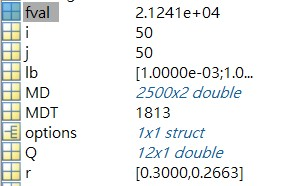
\includegraphics[scale=1]{./graph/result.jpg}
\end{figure}



最後繪製其設計空間、可行解空間與目標函數值,程式有點冗長寫在主程式14-62行。
\begin{figure}[h]
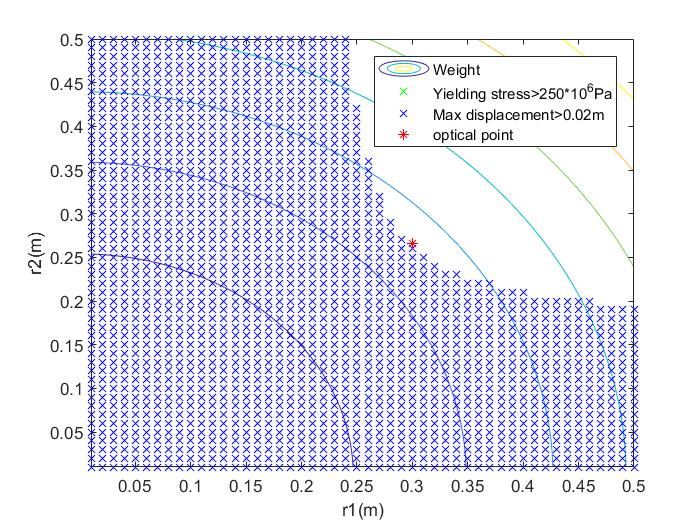
\includegraphics[scale=0.5]{./graph/space.jpg}
\end{figure}

\clearpage



\end{CJK}
\end{document}
